% Tablero Kanban del Proyecto (GitHub Projects), estado al 22 de octubre de 2026.
\begin{figure}[ht]\centering
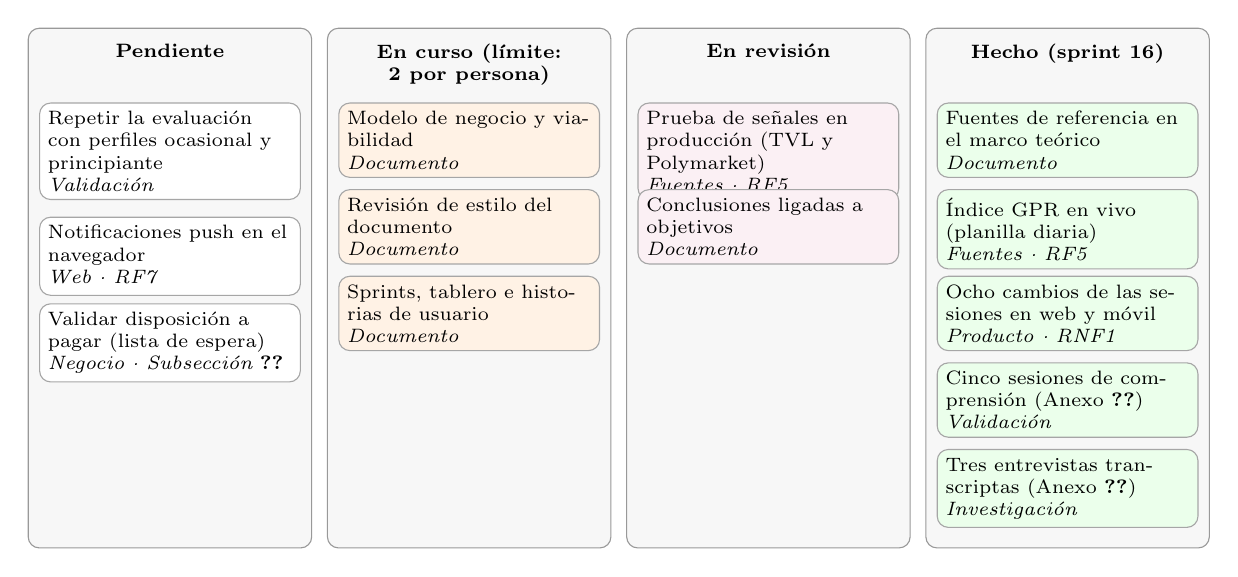
\begin{tikzpicture}[font=\scriptsize,
  col/.style={draw=black!40,rounded corners,fill=black!3,minimum width=3.6cm,minimum height=6.6cm,anchor=north},
  hdr/.style={font=\scriptsize\bfseries,anchor=north},
  card/.style={draw=black!35,rounded corners,fill=white,text width=3.1cm,align=left,inner sep=3pt,anchor=north},
  done/.style={card,fill=green!8},rev/.style={card,fill=purple!6},wip/.style={card,fill=orange!10}]
\foreach \x/\n in {0/Pendiente,3.8/En curso (límite: 2 por persona),7.6/En revisión,11.4/Hecho (sprint 16)}{
  \node[col] at (\x,0) {};\node[hdr,text width=3.3cm,align=center] at (\x,-0.08) {\n};}
% Pendiente
\node[card] (p3) at (0,-0.95) {Repetir la evaluación con perfiles ocasional y principiante\\\textit{Validación}};
\node[card] (p5) at (0,-2.4) {Notificaciones push en el navegador\\\textit{Web · RF7}};
\node[card] (p6) at (0,-3.5) {Validar disposición a pagar (lista de espera)\\\textit{Negocio · Subsección~\ref{sec:viabilidad}}};
% En curso
\node[wip] at (3.8,-0.95) {Modelo de negocio y viabilidad\\\textit{Documento}};
\node[wip] at (3.8,-2.05) {Revisión de estilo del documento\\\textit{Documento}};
\node[wip] at (3.8,-3.15) {Sprints, tablero e historias de usuario\\\textit{Documento}};
% En revisión
\node[rev] at (7.6,-0.95) {Prueba de señales en producción (TVL y Polymarket)\\\textit{Fuentes · RF5}};
\node[rev] at (7.6,-2.05) {Conclusiones ligadas a objetivos\\\textit{Documento}};
% Hecho
\node[done] at (11.4,-0.95) {Fuentes de referencia en el marco teórico\\\textit{Documento}};
\node[done] at (11.4,-2.05) {Índice GPR en vivo (planilla diaria)\\\textit{Fuentes · RF5}};
\node[done] at (11.4,-3.15) {Ocho cambios de las sesiones en web y móvil\\\textit{Producto · RNF1}};
\node[done] at (11.4,-4.25) {Cinco sesiones de comprensión (Anexo~\ref{annex:protocolo-usuarios})\\\textit{Validación}};
\node[done] at (11.4,-5.35) {Tres entrevistas transcriptas (Anexo~\ref{annex:entrevistas})\\\textit{Investigación}};
\end{tikzpicture}
\caption{Tablero Kanban del Proyecto al 23 de octubre de 2026, cierre del sprint 16. Fuente: elaboración propia a partir de GitHub Projects.}\label{fig:kanban}
\end{figure}
